
\subsection{Особенности химического поведения орбитальнодефицитных соединений, их связь с электронным строением.}

Метод валентных связей имеет некоторые недостатки. В частности, с помощью данного метода трудно объяснить нарушение правила инертного газа для PCl5 - у фосфора здесь 10
электронов. Метод валентных связей можно рассматривать как выражение идей Льюиса в терминах волновой механики, а по Льюису каждый атом делит электроны с соседним атомом для
достижения полной валентной оболочки с восемью электронами. 



Вместе с тем, известно, что существует довольно много соединений, у которых нарушено правило инертного газа, но они устойчивы. Например, для гексафторсиликат-аниона у кремния 12
электронов, хотя соли с таким анионом очень устойчивы (рис. 1). Встречаются даже экзотические примеры, как силотран (рис. 2). В окружении кремния там 10 электронов. В продукте
реакции взаимодействия нитрата серебра в пиридине с иодом, у иода 10 электронов (рис. 3).

Попытки объяснить строение PCl5 с помощью идей $sp^3d$-гибридизации не выдерживают никакой критики, ведь 3d-орбитали находятся даже выше по энергии, чем 4s. 

Лучше всего такие молекулы рассматривать с позиций метода молекулярных орбиталей. Молекула PCl5 (PF5 тоже) представляет собой тригональную бипирамиду (рис. 4). Из геометрии
понятно, что, вообще говоря, атомы хлора не эквивалентны друг другу, ведь есть три экваториальных атома и два аксиальных атома хлора. Более того, расстояния фосфор-аксиальный хлор
больше, чем фосфор-экваториальный хлор. Кстати, так как молекулы колеблятся, то положение плоскости может измениться, и аксиальные атомы перейдут в экваториальные, или
наоборот. Это псевдопревращения Берри. Из-за колебательных процессов, реально атомы усредняются и становятся одинаковыми.

Если рассмотреть взаимодействие фосфора с тремя экваториальными атомами хлора, то видно, что у каждого хлора становится по 8 электронов, а у фосфора остаётся ещё одна pz-орбиталь
и ещё два своих электрона (рис. 5). На оставшуюся систему из фосфора и двух аксиальных атомов хлора приходится 3 орбитали и 4 электрона. Понятно, что существует только три
комбинации перекрытия трёх орбиталей (рис. 6). Это связывающая и разрыхляющая орбитали, но есть ещё несвязывающая орбиталь. Получается, что из симметрии «место» для такой
орбитали в молекуле нашлось, и молекула может удерживать там электроны, хоть они и не вносят никакого вклада в связывание - «сколько выиграли, столько и проиграли». Так как 3 атома
удерживаются только 2 электронами (на связывающей орбитали), то связь длиннее. Естественно, что электроны можно расставить только так, как показано на рис. 7. В итоге имеем, что у
атома фосфора недостаточно орбиталей. Поэтому такие соединения называются орбитальнодефицитными электроноизбыточными. 

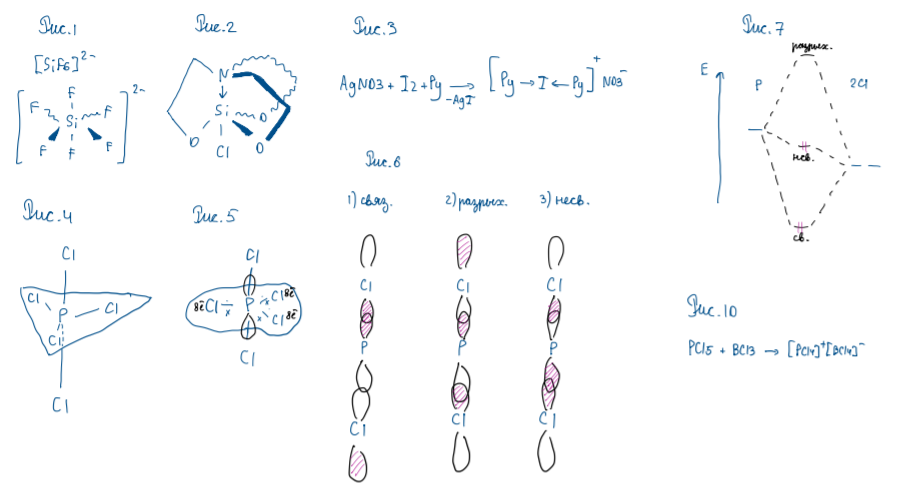
\includegraphics{images/15v1.png}

Диаграмма МО, учитывающая пять орбиталей фтора в PF5, направленные к атому фосфора, приведена на рис. 8.

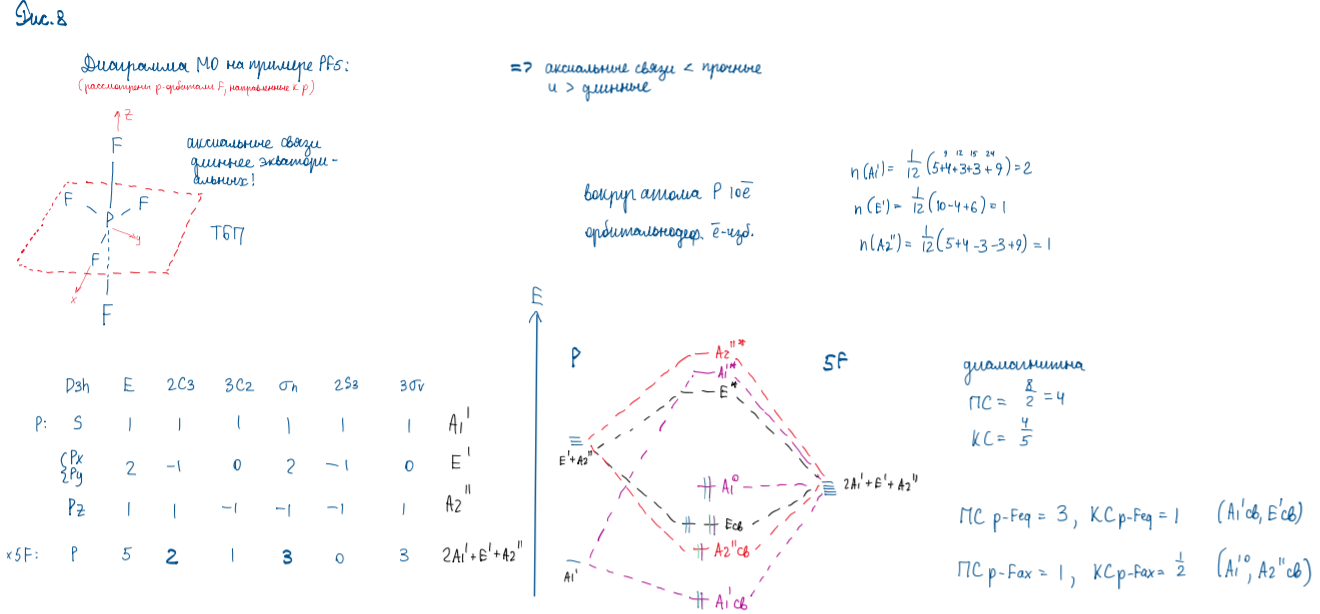
\includegraphics[scale=0.8]{images/15v2.png}


Заметим, что три комбинации перекрывания орбиталей существует и для центральных атомов с s-орбиталью, например, в HF2-. Это очень устойчивый молекулярный ион, хоть у водорода 4
электрона (правило инертного газа для него - 2 электрона). Диаграмма МО для такого аниона представлена на рис. 9. В вышеупомянутом гексафторсиликат-ионе (октаэдрическое строение)
имеется три (по каждой оси) таких 3с4е-взаимодействия

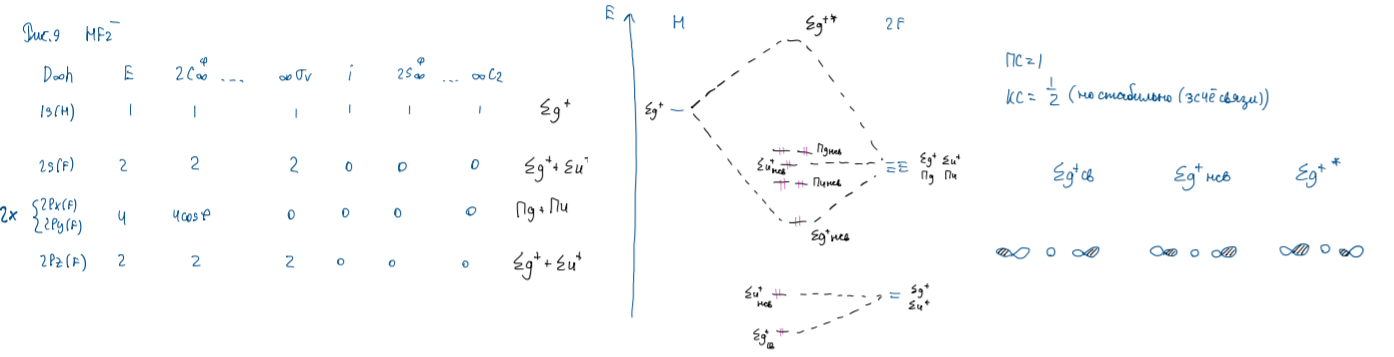
\includegraphics[scale=0.75]{images/15v3.png}

Из вышеперечисленных особенностей электронного строения следуют некоторые химические особенности. Такие молекулы являются основаниями Льюиса, то есть, донорами электронной
пары. Во-первых, если молекула отдаст электронную пару с несвязывающей орбитали, порядок её связывания не изменится. Во-вторых, если у молекулы было 10 электронов (тот же PCl5),
то в результате образуется очень устойчивая восьмиэлектронная система. Пример реакции:

$$PCl_5 + BCl_3 \rightarrow [PCl_4]^+[BCl_4]^-$$

